\documentclass[a4paper,10pt]{article}

\usepackage{graphicx}
\usepackage[utf8]{inputenc}
\usepackage[spanish]{babel}
\usepackage{hyperref}
\usepackage{listings}
\usepackage{verbatim}
\usepackage[top=2cm, bottom=1.5cm, left=2.5cm, right=1cm]{geometry}
\usepackage{pdfpages}
\usepackage{enumitem}
\usepackage{float}
\usepackage{array}
\title{		\textbf{Trabajo Práctico Grupal}}

\author{	Lucas Simonelli, \textit{Padrón Nro. 93111}                     \\
            \texttt{ lucasp.simonelli@gmail.com }                                              \\[2.5ex]
            Tomás Boccardo, \textit{Padrón Nro. 93637}                     \\
            \texttt{ tomasboccardo@gmail.com}                                              \\[2.5ex]
            Andrés Sanabria, \textit{Padrón Nro. 93403}                     \\
            \texttt{ andresg.sanabria@gmail.com  }                                              \\[2.5ex]
            Damián Manoff, \textit{Padrón Nro. 93169}                     \\
            \texttt{ damianmanoff@gmail.com  }                                              \\[2.5ex]
            Gonzalo Beviglia, \textit{Padrón Nro. 93144}                     \\
            \texttt{ gonchu.b@gmail.com  }                                              \\[2.5ex]
            Federico Quevedo, \textit{Padrón Nro. 93159}                     \\
            \texttt{ federico1245@hotmail.com  }                                              \\[2.5ex]
            Joaquín Stankus, \textit{Padrón Nro. 93143}                     \\
            \texttt{ joaquinstan@gmail.com  }                                              \\[2.5ex]
            Nicolás Andrés Gallinal, \textit{Padrón Nro. 88212}                \\
            \texttt{ nicoabie@gmail.com }                                              \\[2.5ex]
            Elías Joel Pringles, \textit{Padrón Nro. 95380}                \\
            \texttt{ elo94@outlook.com }                                              \\[2.5ex]   
          Erwan Le Fur Darmon								               \\
            \texttt{ erwan.le-fur@ensam.eu }                                              \\[2.5ex]   
Valentino Portnoy, \textit{Padrón Nro. 93450}                     \\
            \texttt{ vnportnoy@gmail.com  }                                              \\[2.5ex]
            \normalsize{2do. Cuatrimestre de 2013}                                      \\
            \normalsize{71.12, Estructura de las organizaciones}  \\
            \normalsize{Facultad de Ingeniería, Universidad de Buenos Aires}            \\
       }
\date{}
\begin{document}





\maketitle
\thispagestyle{empty}   % quita el nómero en la primer página


\newpage
\tableofcontents
\newpage
\section{Introducción}
El trabajo consiste en el análisis de las estructuras en distintas organizaciones, tratando de reconocer que módelo teórico se ajusta mejor a cada caso.

En primer lugar se detallará la selección de una empresa para relevar en base a determinados criterios de puntuación. Se eligirá la empresa cuya valorización luego de sumar todos los valores fue la mayor.

A continuación, se realizará un análisis completo de las características principales, relevando las funciones de los cargos principales y confeccionando el manual. Para que esto sea posible, se recurrirá a una serie de reuniones con un representante de la empresa, que proporcionará la información.

Se buscarán dificultades consecuencia de la estructura y se propondrá una mejora.

Finalmente, se estudiarán ciertos casos que presentan distintas problemáticas en determinadas organizaciones y se propondrán posibles soluciones a los problemas.

\newpage
\section{Selección de la empresa}

\subsection{Criterio de seleccion}

Para seleccionar la empresa a relevar, se tuvieron en cuenta las siguientes caracteristicas de cada empresa candidata:

\begin{itemize}
\item Calidad de \emph{Contacto}. 
\item \emph{Localización}.
\item \emph{Tamaño}.
\item \emph{Documentación}. 
\end{itemize}

Se realizó un cuadro comparativo de las empresas que se construye bajo la base de que cada categoría (de las antes descriptas) tiene una valoración fija, determinada por la cátedra. En orden descendente tenemos, como categoría más importante, al contacto (10), seguido por la localización (8), luego el tamaño de la empresa (7) y, por último, la documentación que la empresa pueda presentarnos (6).

La confección del cuadro se realiza estimando, del uno al diez, que puntaje alcanza cada empresa en cada categoría. El puntaje es otorgado por el integrante del grupo que presenta a la empresa como candidata para el trabajo práctico, entendiendo que es quien mayor conocimiento tiene acerca de la misma y puede llegar a un puntaje más acertado.

\subsection{Asignación de puntajes}

\begin{itemize}

\item \textbf{Tecin S.A.: 8.29}\\
\\
\textit{Contacto - 9:}
El tio de un integrante del grupo es director de la empresa. De vez en cuando esta de viaje, pero dentro de todo es accesible.

\textit{Localización - 7:}
La fabrica se ubica en Munro. La dirección de la misma es Gobernador Emilio Castro 3365, Carapachay, Vicente López, provincia de Buenos Aires. Es cercana a la gran mayoría de los integrantes del grupo.

\textit{Documentacion - 10:}
Organigrama actualizado agosto 2013. La empresa está certificada IRAM ISO 9001:2008.

\textit{Tamaño - 7:}
Tiene alrededor de 50 empleados

\item \textbf{Helados Pablo: 5.87} \\
\\
\textit{Contacto - 10:}
El dueño, Pablo, es el tío de uno de los integrantes, el cuál trabajó en la heladería varias temporadas y conoce todo el funcionamiento.

\textit{Localización - 7:}
La central de producción se encuentra en Berazategui, pero la sucursal más importante está en Quilmes, ubicada en zona de altas ventas.

\textit{Documentacion - 2:}
No posee una documentación actualizada ya que el flujo de trabajo depende de la temporada. En baja temporada cambia la mayoría del personal

\textit{Tamaño - 2:}
En temporada alta el tamaño supera los 50 empleados, pero en temporada baja no supera los 15.

\item \textbf{Kimberly-Clark: 4.9} \\
\\
\textit{Contacto - 4:}
Uno de nosotros es pasante en la división de IT para latinoamérica, con poco contacto con las otras divisiones mas relacionadas con la estructura manufacturera.

\textit{Localizacion - 6:}
Hay plantas en Bernal y Pilar, aunque existen oficinas en Puerto Madero y el centro.

\textit{Documentacion - 10:}
Certifican ISO 14001, que pide tener la documentacion en orden.

\textit{Tamaño - 2:}
Es una empresa demasiado grande, con cerca de 1400 empleados.


\item \textbf{Tecna: 7.03} \\
\\
\textit{Contacto - 8:}
Un integrante del grupo trabaja en la empresa. Contaría con el acceso a la información requerida para el trabajo práctico.

\textit{Localización - 10:}
La empresa esta ubicada en Puerto Madero a 5 cuadras de la sede de Paseo Colón, donde la mayoría cursamos.

\textit{Documentacion - 7:}
Organigrama actualizado en Abril 2013. Certificaciones ISO 9001:2008, ISO 14001: 2004 y OHSAS 18001: 2007.

\textit{Tamaño - 5:}
La empresa cuenta con alrededor de 400 empleados en Argentina y 200 mas distribuidos por sus 6 sedes en España, Perú, Bolivia,Colombia , Brasil y Ecuador

\item \textbf{Gamar: 5.55} \\
\\
\textit{Contacto - 8:}
Un integrante del grupo conoce al dueño de la empresa, el cual mostró interés en colaborar.

\textit{Localización - 4:}
La empresa está localizada en el límite entre Tigre y San Fernando. Esta ubicación nos queda lejos a la mayoría de los integrantes.

\textit{Documentacion - 5:}
No presenta organigrama actualizado, pero si cuenta con certificaciones ISO y para las distintas automotoras a las cuales provee de partes.

\textit{Tamaño - 6:}
La empresa cuenta con alrededor de 120 empleados en su planta de producción.


\end{itemize}


\subsection{Resultados}

\newcolumntype{x}[1]{%
>{\centering\hspace{0pt}}p{#1}}%
\begin{table}[!htbp]\centering
\begin{tabular}{|x{3cm}|x{2cm}|x{2cm}|x{2cm}|x{2cm}|x{2cm}|x{2cm}|}
\cline{1-7}
  & \textbf{Valoración} & \textbf{Tecin} & \textbf{Helados Pablo} & \textbf{Kimberly-Clark} & \textbf{Tecna} & \textbf{Gamar} \tabularnewline
\hline
\textbf{Contacto} & 10 & 10 & 10 & 4 & 8 & 8\tabularnewline 
\hline
\textbf{Localización} & 8 & 6 & 7 & 6 & 10 & 4\tabularnewline 
\hline
\textbf{Documentación} & 6 & 10 & 2 & 10 & 8 & 5\tabularnewline 
\hline
\textbf{Tamaño} & 7 & 7 & 2 & 2 & 5 & 6\tabularnewline 
\hline
 \multicolumn{2}{|c|}{\textbf{Total}} & 8,29 & 5,87 & 4,90 & 7,03 & 5,55\tabularnewline
\hline
\end{tabular}
\end{table}

La empresa con mayor puntaje, y sobre la cual realizamos el trabajo práctico, fue \textbf{Tecin S.A}.
\newpage
\section{Empresa relevada}
	\subsection{Preguntas}
		\subsubsection{Preguntas introductorias}
			\begin{enumerate}
				\item \textit{¿Cuál es la razón social de la empresa?}\\
				Tecnología Contra Incendios S.A.
				
				\item \textit{¿En qué lugar se encuentra localizada la empresa?}\\
				La empresa está ubicada en Carapachay, Munro. La dirección es Gobernador Emilio Castro 3365.			
				
				\item \textit{Mencione los acontecimientos más destacados en la evolución de la empresa.}\\
				La empresa nace en el año 1965, bajo el nombre de \textbf{TECIN ARGENTINA S.R.L.} Al poco tiempo se transforma en una S.A. y obtiene la representación y distribución, de empresas internacionales de reconocida trayectoria en su especialidad como Rosenbauer, Angus, Reliable, Walter Kidde, Total y Cerberus. En 1982 la empresa construye la primer autobomba argentina tras asociarse con la empresa austriaca Rosenbauer K.G. (hoy Rosenbauer International A.G.).\\
				En la década del 90, sus accionistas deciden formar sociedades independientes para atender unidades de negocios y mercados diferentes, siendo una de ellas: 
				\begin{itemize}
					\item \textbf{Tecnología Contra Incendios S.A.}, es hoy 100\% propiedad de accionistas argentinos y esta dedicada a la fabricación de vehículos y equipos contra incendios y rescate.
				\end{itemize}
				\item \textit{¿Cuál es el rubro al que se dedica la empresa?}\\
				Equipos de seguridad contra incendios (vehículos/equipos/herramientas).
			
				\item \textit{¿Cuál es la línea de productos ofrecida por la organización?}\\	
				La línea de productos ofrecida es de:\\
				\textbf{Vehículos}:
				\begin{itemize}
					\item Contra incendios urbanos, industriales y forestales.
					\item De rescate y manejo de sustancias peligrosas.
				\end{itemize}
				\textbf{Productos/equipos}:
				\begin{itemize}
					\item Motobombas portátiles.
					\item De protección personal y respiratoria.
					\item Para controlar incendios: mangueras, matafuegos, etc.
				\end{itemize}	
												
				\item \textit{¿La empresa cumple algún tipo de certificación?}\\
				Sí, la empresa está certificada bajo las normas IRAM ISO 9001:2008
						
			\end{enumerate}
			
			
		\subsubsection{Comercial}
		
		
			\begin{enumerate}[resume]
			
				\item \textit{¿Cuáles son los productos más vendidos por la empresa?}\\
				El producto más vendido por la empresa son las autobombas para combate de incendio urbano.
				
				\item \textit{¿Qué productos son exportados por la empresa?}\\
				Los productos exportados por la empresa son las autobombas producidas.
				
				\item \textit{¿Cuáles son los principales destinos de las exportaciones?}\\
				Los principales destinos de las exportaciones son los países de Sudamérica.
				
				\item \textit{¿Qué porcentaje del mercado concentran los productos fabricados?}\\
				En el interior, la empresa concentra el 30\% del mercado.
				
				\item \textit{¿Qué métodos de publicidad utiliza la empresa?}\\
				Los métodos de publicidad que emplea la organización son:
				\begin{itemize}
					\item Avisos en revistas especializada
					\item Exposiciones
					\item Campañas de emailing
				\end{itemize}
				
				\item \textit{¿Cuáles son los principales clientes de la empresa?}\\
				Entre los principales clientes de TECIN se encuentran:
				\begin{itemize}
					\item Estado Nacional
					\item Cerro Vanguardia
					\item Cerro Negro
					\item Sipetrol
				\end{itemize}
				
				\item \textit{¿Cómo se planifica la distribución de los pedidos?}\\	
				La planificación de la distribución de los pedidos se realiza en la etapa de producción y se utiliza el criterio \'First In, First Out\'.
				
			\end{enumerate}
			
\subsubsection{Producción}
			\begin{enumerate}[resume]
				\item \textit{¿En qué consiste el proceso productivo del producto principal?}\\	
				El proceso de producción de las autobombas urbanas consta de las siguientes etapas:
				\begin{itemize}
					\item \textbf{Ensamblado del chasis}: El chasis arriba a las instalaciones desarmado, por lo que hay que ensamblarlo en una única parte.
					\item \textbf{Integración de los ejes con el chasis}: Los ejes trasero y delantero son integrados al chasis.
					\item \textbf{Colocación de la carrocería}: Se coloca la carrocería sobre el chasis.
					\item \textbf{Colocación de equipos contra incendios}: Se colocan las bombas de agua, motores y válvulas que permiten al vehículo desempeñarse en su tarea.
					\item \textbf{Pintura exterior y acabado interior}: Se pinta la carrocería y partes interiores. Se colocan butacas y accesorios adicionales.
				\end{itemize}
				
				
				\item \textit{¿Cuáles son las principales materias primas?}\\	
				Las principales materias primas utilizadas en la producción son las siguientes:
				\begin{itemize}
					\item Chapa de acero
					\item Chapa de aluminio
					\item Pintura
					\item Componentes mecánicos
				\end{itemize}
				
				\item \textit{¿Cuáles son los proveedores más importantes de la empresa?}\\	
				Los principales proveedores de la empresa son:
				\begin{itemize}
					\item Ford
					\item Mercedes Benz
					\item VolksWagen
					\item Estusora Argentina
					\item TER
					\item DER
					\item Pinturerias Varias
				\end{itemize}
				
				\item \textit{¿Produce algún insumo necesario para la manufactura del producto final?}\\	
				No, la empresa no produce ninguno de los insumos necesarios.
				
				\item \textit{¿Poseen un equipo que se encargue del mantenimiento, o es un servicio tercerizado?}\\	
				La empresa tiene un equipo especializado en el mantenimiento de sus productos.
				
				\item \textit{¿Necesita operarios calificados?}\\	
				Si, algunos procesos puntuales de la producción requieren operarios calificados.
				
				\item \textit{¿Qué insumos son importados por la organización?}\\	
				Los insumos importados son:
				\begin{itemize}
					\item Bombas de agua
					\item Mangueras
					\item Cortinas de aluminio
				\end{itemize}
			
			\end{enumerate}			
			
	\subsubsection{R.R. H.H.}
		
		
			\begin{enumerate}[resume]

			\item \textit{¿Cuántos empleados tiene la organización?}\\
			La empresa tiene 50 empleados.
				
			\item \textit{¿Qué beneficios posee el personal de la empresa?}\\
			Los principales beneficio ofrecidos para el personal son:
			\begin{itemize}
				\item Comedor
				\item Medicina Prepaga
				\item Planes de capacitación
				\item Bono anual atado a resultados				
			\end{itemize}
			
			\item \textit{¿Cuáles son los principales sectores de la empresa?}\\
			Los principales sectores de la empresa son:
			\begin{itemize}
				\item Administración y Finanzas
				\item Abastecimiento
				\item Ventas
				\item Producción
				\item Servicios
			\end{itemize}
			
			\item \textit{¿Tiene la empresa un organigrama propio?}\\
			Si, la empresa posee organigrama propio.
					
			\item \textit{¿Puede la empresa proporcionar dicho organigrama?}\\
			Si, la empresa puede proporcionar dicho organigrama
			
			\item \textit{¿Cómo es el proceso de selección del personal? }\\
			La empresa contrata a una consultora que se encarga de publicar los avisos y realizar una preselección de los postulantes. Una vez entregada la preselección, la organización se encarga de realizar otra etapa de entrevistas para decidir que postulante es el más capacitado. Una vez seleccionado, el postulante debe realizar un estudo psicotécnico con potencial de desarrollo, un estudio preocupacional y si todos los resultados son correctos se realiza el alta temprana.

			\item \textit{¿Se realizan evaluaciones periódicas del desempeño del personal?}\\
			La organización realiza evaluaciones de desempeño semestrales a todo su personal
			
			\item \textit{¿Hay bonificaciones salariales por buen desempeño?}\\
			Las bonificaciones que ofrece la empresa son por buen desempeño, pero atadas a resultados.
			
			\item \textit{¿Se realizan capacitaciones periódicas a los empleados?}\\
			Si, los empleados tienen un programa de capacitaciones periódicas como parte de sus beneficios
			
			\item \textit{¿Se organizan eventos para fomentar la relación interpersonal entre los empleados?}\\
			No, la organización no organiza eventos.
			
			\item \textit{¿Contratan servicios tercerizados, como por ejemplo: estudio contable, jurídico, controles de calidad, etc.?}\\
			Si, se contrata a un estudio contable para la liquidación de sueldos y para realizar auditorias.			

			\end{enumerate}
			
			
		\subsubsection{Finanzas}
		
		
			\begin{enumerate}[resume]
			
			\item \textit{¿Cuáles son los plazos promedio para la cobranza de las facturas?}\\
			El plazo promedio de la cobranza de las facturas es de 60 días.
			
			\item \textit{¿Recibe algún beneficio impositivo por parte del estado?}\\
			No, la empresa no recibe ningún beneficio impositivo.
			
			\end{enumerate}
		
		\subsubsection{Control de Calidad}
		
		
			\begin{enumerate}[resume]

			\item \textit{¿Cuáles es la política de calidad de la organización?}\\
			La política de calidad de la empresa presenta los siguientes objetivos:
			\begin{itemize}
				\item El cumplir con los compromisos contraídos con los clientes y superar sus expectativas, constituyen una obligación para todo el personal.
				\item Asumir como  indispensable el cumplimiento  de los requerimientos del Sistema de 
Gestión  de la Calidad y comprometerse a su continua mejora.
				\item Nos comprometerse a evaluar, motivar y capacitar a los recursos humanos, en forma 
permanente. 
				\item Mantener un contacto productivo con los Proveedores, para mejorar las prestaciones 
y productos ofrecidos. 
				\item Difundir al personal los objetivos comprometidos en la presente política. 
			\end{itemize}
	
			\item \textit{¿Cómo realizan los controles de calidad sobre la producción?}\\			
			El control de calidad es interno. Se realiza en cada una de las etapas de la producción
			
			\item \textit{¿Realizan auditorías internas? ¿Con qué frecuencia?}\\
			Si, la empresa tiene un cronograma de auditorias. Pueden ser mensuales o bimestrales.
			
			\item \textit{¿Realizan auditorías externas? ¿Con qué frecuencia?}\\			
			Si, se realizan auditorias a proveedores y contratistas a necesidad, aunque también existe un cronograma de auditorias.
			
			\end{enumerate}
	\subsection{Minuta de Reunión 02/09/2013}
\hyphenation{fa-mi-li-ar} 
\begin{flushleft}
	\begin{tabular}{|p{15cm}|}
		\hline
		\textbf{Fecha:} 02/09/2013 \\ \hline
		\textbf{Duración de la entrevista:} 40 minutos\\ \hline
		\textbf{Lugar:} TECIN S.A.\\ \hline
		\textbf{Presentes:} \\
			Por parte de la empresa: Daniel Abé, Director General de TECIN S.A. \\ 
			Por parte del grupo: Tomás Boccardo \\ \hline
	\end{tabular}  \\
	\vspace{0.7cm}
	\begin{tabular}{|p{15cm}|}
		\hline
		\textbf{Síntesis de los temas tratados:}\\
		\hline
		\begin{itemize}
			\item \textbf{Historia de la empresa:}
			Se conversó sobre la fundación en 1965 bajo en nombre de TECIN SRL, representación de empresas internacionales a lo 				largo de su historia, historia de su producción, principales socios y sobre la división de la empresa en la década 					del 90.

		\item \textbf{Organización de la empresa:} 
		Se le solicitó al encuestado el organigrama de la empresa.

		\item \textbf{Principales productos:} La empresa se dedica principalmente a producir autobombas para 
		la utilización urbana, forestal, aeroportuaria, entre otros sectores. Además se producen insumos y repuestos para el 				combate y la prevención de incendios, tanto forestales como urbanos.
		
		\item \textbf{Recorrido por las instalaciones de la fabrica}

		\end{itemize} \\ \hline
	\end{tabular} \\
	\vspace{0.7cm}
	\begin{tabular}{|p{15cm}|}                
		\hline 
		\textbf{Distribuir a:} presentes, Ing. Veber\\
		\hline
		\textbf{Próxima entrevista:} Fecha a determinar\\
		\hline
	\end{tabular}	
	
\end{flushleft}
	\subsection{Minuta de Reunión 26/09/2013}
\hyphenation{fa-mi-li-ar} 
\begin{flushleft}
	\begin{tabular}{|p{15cm}|}
		\hline
		\textbf{Fecha:} 26/09/2013 \\ \hline
		\textbf{Duración de la entrevista:} 40 minutos\\ \hline
		\textbf{Lugar:} San Antonio de Areco\\ \hline
		\textbf{Presentes:} \\
			Por parte de la empresa: Daniel Abé, Director General de TECIN S.A. \\ 
			Por parte del grupo: Tomás Boccardo \\ \hline
	\end{tabular}  \\
	\vspace{0.7cm}
	\begin{tabular}{|p{15cm}|}
		\hline
		\textbf{Síntesis de los temas tratados:}\\
		\hline
		\begin{itemize}
			\item \textbf{Cuestionario de presentación:}
			Se realizaron las preguntas de presentación de la empresa. Se trataron temas sobre las áreas Comercial, Producción, RR.HH., Finanzas y Control de calidad.

		\item \textbf{Comentarios y dudas sobre el organigrama:} 
		Se le plantearon al entrevistado los comentarios y las dudas que surgieron en el grupo al discutir el organigrama.

		\item \textbf{Propuesta de mejora al organigrama:} El entrevistado colaboró con su punto de vista para plantear una posible mejora o modificación al organigrama enseñado.

		\end{itemize} \\ \hline
	\end{tabular} \\
	\vspace{0.7cm}
	\begin{tabular}{|p{15cm}|}                
		\hline 
		\textbf{Distribuir a:} presentes, Ing. Veber\\
		\hline
		\textbf{Próxima entrevista:} Fecha a determinar\\
		\hline
	\end{tabular}	
	
\end{flushleft}
	\subsection{Minutas de Reunión 26/09/2013}
\hyphenation{fa-mi-li-ar} 
\begin{flushleft}
	\begin{tabular}{|p{15cm}|}
		\hline
		\textbf{Fecha:} 29/10/2013 \\ \hline
		\textbf{Duración de la entrevista:} 20 minutos\\ \hline
		\textbf{Lugar:} Conversación telefónica\\ \hline
		\textbf{Presentes:} \\
			Por parte de la empresa: Daniel Abé, Director General de TECIN S.A. \\ 
			Por parte del grupo: Tomás Boccardo \\ \hline
	\end{tabular}  \\
	\vspace{0.7cm}
	\begin{tabular}{|p{15cm}|}
		\hline
		\textbf{Síntesis de los temas tratados:}\\
		\hline
		\begin{itemize}
			\item \textbf{Propuesta de mejora del organigrama:}
			Se plantearon dudas que surgieron a partir de la corrección de la propuesta presentada anteriormente. Se realizo la propuesta de separar el área de Administración y Finanzas. Se discutió sobre los posibles beneficios. El contacto concordó con la propuesta.

		\item \textbf{Consultas sobre funciones enviadas:} 
		Se le plantearon al entrevistado las dudas que surgieron al discutir con el grupo las funciones que el contacto había enviado con anterioridad.

		\item \textbf{Agradecimientos:} Se agradeció al entrevistado su ayuda para poder realizar este informe

		\end{itemize} \\ \hline
	\end{tabular} \\
	\vspace{0.7cm}
	\begin{tabular}{|p{15cm}|}                
		\hline 
		\textbf{Distribuir a:} presentes, Ing. Veber\\
		\hline
		\textbf{Próxima entrevista:} Fecha a determinar\\
		\hline
	\end{tabular}	
	
\end{flushleft}
	
	\subsection{Organigrama relevado}
	Gracias a los datos provistos por el contacto, se pudo relevar el siguiente organigrama de la empresa en donde se ven las unidades organizativas principales.
	\begin{figure}[H]
		\centering
		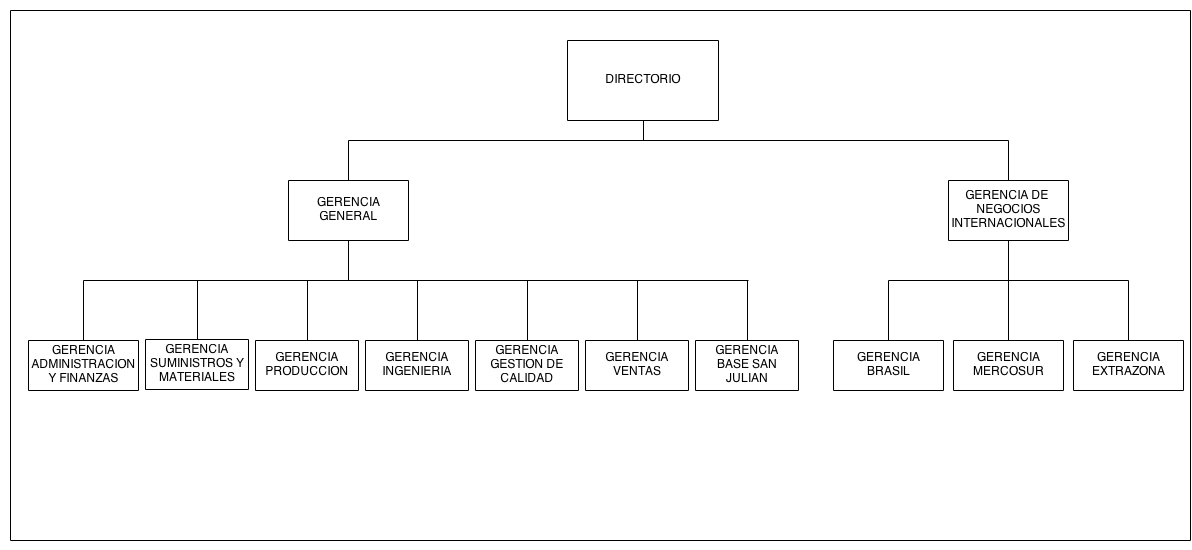
\includegraphics[width=15cm]{imagenes/actualOrganigrama.png}
		\caption{Organigrama actual TECIN S.A.}
	\end{figure}
	A partir de este organingrama, y con la información provista por el entrevistado, se relevaron las funciones de cada una de las unidades organizativas de la empresa.
		\subsubsection{Gerencia General}
			Conducir, organizar, articular, supervisar y controlar el desarrollo de los procesos de gestión de las unidades orgánicas a su cargo.
			Autoridad sobre: gerencia operaciones, gerencia ventas, y todas las demás subgerencias.
			\paragraph{Administración y Finanzas:}
			Planificar, dirigir y controlar la administración financiera, de personal y de los activos de la empresa, a través de sistemas de presupuesto, información contable, tesorería, administración y mantenimiento de los bienes físicos.
			Contribuir al cumplimiento de las disposiciones legales y a la toma de decisiones, mediante la confección de estados contables, liquidaciones impositivas 
			\paragraph{Suministros y Materiales:}
			Asegurar el abastecimiento de componentes y materias primas a la línea de
producción, tanto nacionales como de importación, como así también insumos,
consumibles y bienes necesarios para el normal funcionamiento de la empresa.
Asegurar que los elementos a producir sean realizados dentro de los plazos
contractuales y al costo previsto al momento de su oferta.
			\paragraph{Producción:}
			Lograr la producción de equipos y vehículos, como también la prestación de servicios
internos, instalación y/o mantenimiento de sistemas Ansul R-102, comprometidos con los
Clientes, en un todo de acuerdo a los requerimientos contractuales, los niveles de calidad,
seguridad y en los plazos acordados en la programación, dentro del marco de políticas y
procesos autorizados, y de acuerdo a los diseños transferidos por el área de ingeniería,
mediante la asignación de recursos a los distintos sectores productivos, una adecuada
planificación y un efectivo control de la producción y asignación de mano de obra.
			Coordinar los proyectos desde el momento de su cotización y en la etapa de producción,
garantizando que los mismos sean ejecutados cumpliendo los plazos contractuales y al costo
previsto.
			\paragraph{Ingeniería:}
			Desarrollar estudios de costos con alto grado de detalle, especificaciones y planos de
oferta para la cotización de los productos producidos por la empresa.
Desarrollar soluciones de transmisiones cardanicas para el accionamiento de
bombas de incendios.
			\paragraph{Gestión de calidad:}
			Dirigir, planificar, organizar y controlar los procesos, procedimientos y actividades relacionados con la gestión de la calidad, con el fin de garantizar el cumplimiento de sus estándares y normas, así como, favorecer la mejora continua.
			\paragraph{Gerencia ventas:}
			Autoridad: no se relevó.

			Planificar, organizar, dirigir, controlar y coordinar eficientemente el sistema comercial,
diseñando estrategias que permitan el logro de los objetivos empresariales, dirigiendo el
desarrollo de las actividades de marketing y las condiciones de venta de los servicios postales
y afines.
			\paragraph{Base San Julian:}
			Llevar adelante los servicios prestados por la empresa en las instalaciones del Cliente, garantizando las condiciones de calidad establecidas, condiciones seguras de trabajo para el personal a cargo, generando valor y fortaleciendo la imagen de la empresa frente al Cliente.
		\subsubsection{Negocios Internacionales}
			Planificar, organizar, dirigir, controlar y coordinar eficientemente las actividades de marketing,
diseñando estrategias que permitan la inserción de la producción de la compañía más allá del territorio nacional.

\subsection{Estructura de la empresa}
El organigrama del sector de producción es el siguiente:
	\begin{figure}[H]
		\centering
		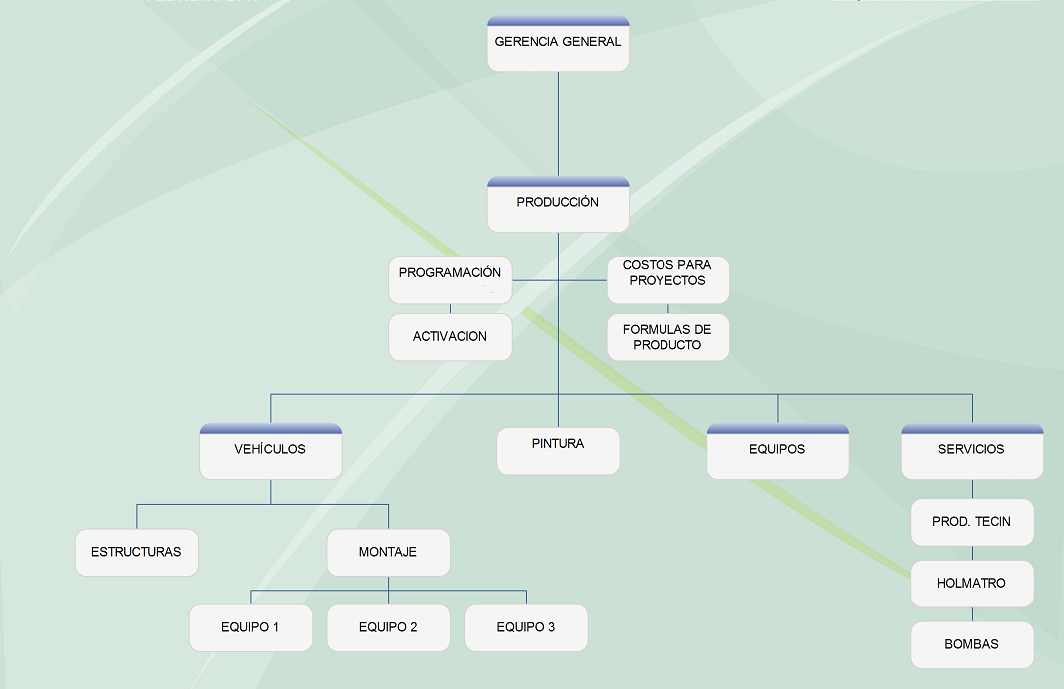
\includegraphics[width=15cm]{imagenes/produccion.png}
		\caption{Organigrama sector producción}
	\end{figure}
Se puede observar que hay una clara diferenciación en áreas especializadas. Sin embargo, éstas no tienen mucha independencia, son controladas
por los niveles superiores en forma estricta. Además vemos que hay un área de servicios. Éste área se encarga de asesorar a las demás. Por lo tanto,
se determina que la estructura formal que más parecido guarda con la empresa relevada es la de línea + staff.

\subsection{Mejora propuesta}
	Luego de analizar y discutir sobre el organigrama provisto por la empresa y teniendo en cuenta los comentarios y sugerencias del contacto, el grupo decidió plantear como mejora la unificación de las áreas de Ingeniería y Producción en una sola gerencia de Operaciones, con el fin de centralizar y facilitar la coordinación de estas dos áreas, logrando así una toma de decisiones más acoplada entre los dos sectores más importantes de la organización. Además, también se planteó la separación del área de Administración y Finanzas en dos áreas independientes para hacer a la diferenciación horizontal  de la compañía y favorecer la especialización. El organigrama resultante es el siguiente:
	\begin{figure}[H]
		\centering
		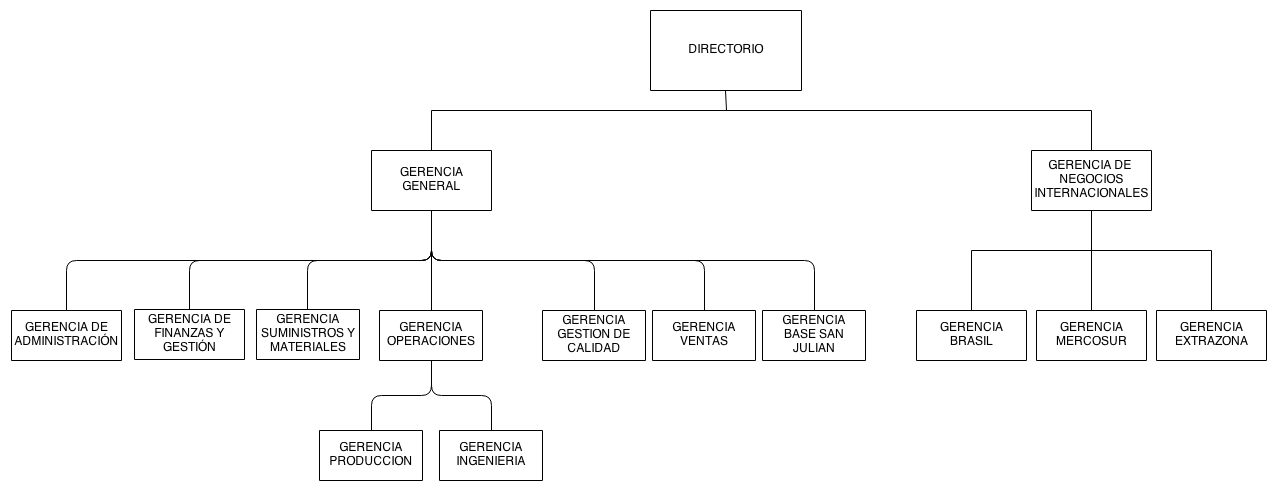
\includegraphics[width=15cm]{imagenes/mejoraOrganigrama.png}
		\caption{Organigrama con mejora propuesta por el grupo}
	\end{figure}
	\paragraph{Administración:}
			Contribuir al cumplimiento de las disposiciones legales y a la toma de decisiones, mediante la confección de estados contables, liquidaciones impositivas.
	\paragraph{Finanzas y Gestión:}
			Planificar, dirigir y controlar la administración financiera, de personal y de los activos de la empresa, a través de sistemas de presupuesto, información contable, tesorería, administración y mantenimiento de los bienes físicos.
	\paragraph{Operaciones:}
			Coordinar los proyectos desde el momento de su cotización y en la etapa de producción e ingeniería,
garantizando que los mismos sean ejecutados cumpliendo los plazos contractuales y al costo previsto.
	\paragraph{Producción:}
			Lograr la producción de equipos y vehículos, como también la prestación de servicios
internos, instalación y/o mantenimiento de sistemas Ansul R-102, comprometidos con los
Clientes, en un todo de acuerdo a los requerimientos contractuales, los niveles de calidad,
seguridad y en los plazos acordados en la programación, dentro del marco de políticas y
procesos autorizados, y de acuerdo a los diseños transferidos por el área de ingeniería,
mediante la asignación de recursos a los distintos sectores productivos, una adecuada
planificación y un efectivo control de la producción y asignación de mano de obra.
\paragraph{Ingeniería:}
			Desarrollar estudios de costos con alto grado de detalle, especificaciones y planos de
oferta para la cotización de los productos producidos por la empresa.
Desarrollar soluciones de transmisiones cardanicas para el accionamiento de
bombas de incendios.
\newpage
\section{Conclusiones}
La presente mejora fue propuesta ante la sugerencia de el contacto, por lo tanto, se supone que será
implementada eventualmente. La empresa es relativamente pequeña todavía, pero los problemas de comunicación
son abundantes, con lo que la mejora favorecerá mucho la coordinación de la producción.

Con respecto al trabajo de relevamiento, se rescata la buena predisposición del contacto, siempre
dispuesto a ayudar al grupo cuando se lo contactó. Desde el primer momento se llegó a un entendimiento
claro, las preguntas realizadas le resultaron claras y las respuestas fueron concisas.
\newpage
\section{Casos de estudio}
	\subsection{Caso 1: Elevadores Hércules S.A.}
		\subsubsection{Enunciado}
		Elevadores Hércules S.A., establecida en Buenos Aires en 1919 como una oficina de
contratistas, se desarrolló al punto de transformarse en una de las compañías más
importantes del mundo. En 1966, la compañía producía 1650 elevadores y en 1974
llegó a 7.850 unidades, inclusive escaleras mecánicas. Aunque su planta principal está
ubicada en Buenos Aires, tiene oficinas comerciales en las 18 ciudades más importantes
del país participando con más del 60\% del mercado nacional. A partir de 1970 el número
de edificios comenzó a aumentar considerablemente. Los pedidos de los clientes tendían
a alcanzar límites que sobrepasaban la capacidad de producción de la fábrica. Los
atrasos en la entrega de pedidos llegaron al punto de provocar serios conflictos entre los
departamentos de ventas y producción.\\
En función de lo anterior, la alta dirección de la compañía decidió perfeccionar el
sistema de planeamiento y control de la fábrica.\\ \\
\textbf{Principales características del sistema de producción}\\
La producción de elevadores requiere cerca de 6.000 diferentes grupos de piezas de
varios tipos o medidas y aproximadamente 12.000 ítems de stock. La mayoría de los
fabricantes depende de sus proveedores para piezas especializadas como por ejemplo
motores eléctricos, cabinas, relees de contacto, guías, puertas metalizas y cerraduras.
Al contrario de esto, elevadores Hércules S.A. tiene la directriz de ser autosuficiente y
producir todas las piezas que utiliza. De esto resulta que la empresa tiene una producción
bastante diversificada, que no es común en su ramo y que da origen a un complejo
sistema de planeamiento y control de la producción.\\
La producción de elevadores no puede seguir un plan general, por que los pedidos
varían considerablemente de acuerdo a las necesidades de los edificios en construcción.
Apenas algunas partes de los elevadores Hércules son Standard y producidas para stock,
como por ejemplo: correderas-guías, guías de puerta, cerradores, motores y conjuntos de
motores generadores, relees de contacto y botones de llamada. El planeamiento de
producción esta dificultado también por el desarrollo tecnológico de la construcción de
diferentes tipos de lugares, dependiendo por eso de condiciones que difícilmente se
pueden prever.\\
El equipo de producción y montaje de elevadores estaba dividido en 4 grupos generales,
de acuerdo con la secuencia a ser seguida en la entrega de partes, conforme al
siguiente esquema:

\begin{itemize}
\item \textbf{Grupo 1}: Modelo soporte para la cabina, guías, correderas, barras, amortiguadores, base, máquina y polea de desvío.
\item \textbf{Grupo 2}: Tablero de comando
\item \textbf{Grupo 3}: Armazón de cabina, contrapesos, paragolpes, plataforma, cabina y cables de acero.
\item \textbf{Grupo 4}: Puertas de lobby, visores, cerraduras, botones de llamada y otros detalles necesarios para que complete el montaje en el edificio.
\end{itemize}

La producción de la fábrica estaba organizada a través de las siguientes secciones:

\begin{enumerate}
\item \textit{Maquinas operativas, tornos, plegadoras, perforadoras, rectificadoras}
\item \textit{Estampado}
\item \textit{Montaje de máquinas}
\item \textit{Montaje de motores}
\item \textit{Montaje de aparatos eléctricos}
\item \textit{Montaje y conexión de cuadros de comando}
\item \textit{Carpintería, fabricación de contrapesos, cabinas y puertas de acero.}
\item \textit{Carpintero, cabinas, puertas y plataformas de madera}
\item \textit{Pintura y galvanoplastia}
\end{enumerate}

En 1970, el planeamiento de producción de elevadores Hércules S.A. era un simple
proceso basado en reportes mensuales de campo del departamento técnico, encargado
del montaje de los elevadores, formado por varios grupos de empleados especializados.
Cada grupo era responsable por el control de una cierta área de la ciudad. El jefe de
grupo visitaba periódicamente a varios clientes de su localidad y estimaba futuras
necesidades. Completaba un formulario de avances del mes donde volcaba los avances
de cada obra indicando el grado de avance de la construcción y estableciendo los
programas de entrega de acuerdo con los cuatro grupos generales del proceso de
producción y montaje ya mencionados. Una vez que el formulario se completaba, le era
entregado al planeador de la producción, un antiguo supervisor que, en 1942, se convirtió
en asistente del departamento de producción a fin de controlar el proceso de
planeamiento de la compañía.\\
A partir de los formularios de avances del mes recibidos por todas las áreas, el
planeador elaboraba el programa de producción para todas las partes a ser producidas
de acuerdo a la secuencia numérica indicada por el departamento de ventas y que
obedecía al orden de entrada de los pedidos de los clientes. El planeador recibía
también las copias de orden de fabricación individual realizadas por el departamento
de ingeniería, conteniendo las especificaciones necesarias para producir cada elevador.
En la época en que la cantidad de elevadores producidos era relativamente baja en
relación con la capacidad de producción de la fabrica, el sistema de planeamiento
descrito, probó ser simple y eficiente y podía ser fácilmente controlado por el planeador
y por los jefes de sección que en conjunto programaban la producción, determinando
cantidades y especificaciones, pidiendo materiales a ser producidos por la fundición, de
oficinas o del pañol.\\
Los reportes mensuales de los grupos de campo eran suficientes para dar al planeador
las informaciones en cuanto a las necesidades futuras de los edificios en construcción y
por lo tanto, esclarecer las prioridades de producción.\\
Entretanto a partir de 1970, el número de construcciones comenzó a aumentar. Los
retrasos en las entregas de elevadores hicieron que los jefes de campo fijasen los
plazos de entrega muy anticipados en sus informes mensuales. Con eso las
informaciones recibidas por el programador fueron perdiendo parte de su valor como
base para la programación. Ocurrió también que ni el planeador ni los jefes de sección
de producción eran avisados cuando un edificio tenía sus obras paralizadas, haciendo
que fuese mantenido el stock de sus correspondientes semielaborados. Este desperdicio
agravaba todavía más la situación de los atrasos provocando graves reclamos por parte
de otros clientes. Teniendo eso en vista, el departamento de ventas comenzó a sugerir
alteraciones en las prioridades distintas a las ordenes de producción, lo que llevo a los
empleados a abandonar los métodos de programación que hasta entonces había sido
establecidos por los jefes de grupo, pasando entonces a trabajar de acuerdo a las
órdenes de ventas del departamento respectivo.\\ \\
\textbf{Decisiones}\\
En vista de la situación, la alta dirección decidió perfeccionar el sistema de planeamiento y control de la fábrica. Contratar una consultora para que analice el caso y revertir la situación de esta compañía.

\subsubsection{Preguntas}
			\begin{enumerate}
		
			\item \textit{ De acuerdo al enfoque de sistemas, caracterizar a la organización de referencia indicando las entradas, las salidas, la retroalimentación y el ambiente}\\

\textbf{Entradas} son los pedidos realizados por los clientes a ventas.\\

\textbf{Proceso} es el conjunto de operaciones unitarias necesarias para modificar las características de las materias primas. Los distintos procesos transforman estas materias primas en un producto final.\\
En este caso particular los distintos procesos son:
\begin{enumerate}
\item Maquinas operativas, tornos, plegadoras, perforadoras, rectificadoras
\item Estampado
\item Montaje de máquinas
\item Montaje de motores
\item Montaje de aparatos eléctricos
\item Montaje y conexión de cuadros de comando
\item Carpintería, fabricación de contrapesos, cabinas y puertas de acero.
\item Carpintero, cabinas, puertas y plataformas de madera
\item Pintura y galvanoplastia
\end{enumerate}
\textbf{Salidas} en una empresa manufacturera son productos, en este caso los ascensores y las escaleras mecánicas.\\

\textbf{Retroalimentación} son las visitas periódicas a clientes y estimar futuras necesidades.\\

\textbf{Ambiente} es el entorno en el que se desarrolla la empresa. Un mercado con demanda en ascenso desde 1970 impulsado por una urbanización orientada a la edificación.

			\item \textit{¿Cúal es el problema evidente que enfrenta la empresa}\\
El notable crecimiento en la demanda de ascensores en el último tiempo, no acompañado de un igual desarrollo de la organización, están provocando que la empresa no pueda responder adecuadamente a tantos pedidos.\\		
			Este incoveniente se ve agravado por la descoordinación entre los departamentos de ventas y planeamiento, impulsada por la falta de control en la información provista por ventas. Esta información al ser errónea y parcial originó serios problemas en el planeamiento de la producción. 
			El departamento de Ventas culpa a Producción de no cumplir con los tiempos establecidos(los cuales están distorsionados para ejercer presión y culpar a Producción de los incovenientes).
			Por su parte, el departamento de Producción se defiende, argumentando que se vende más de lo que se puede producir.
			
			\item \textit{¿Cúal es la parte de la estructura que surge como clave?}\\
			La Tecnoestructura es la parte que surge como clave dado que es el área que debe encargarse de llevar a cabo la estandarización de los procesos de trabajo y de la reaorganización de la estructura. Con estos cambios se puede llegar a conseguir la brecha entre lo que se promete a la hora de la venta y lo que se puede producir realmente.

			\item \textit{¿Cúal es el mecanismo de coordinación preponderante y por qué?}\\
			Actualmente no hay un claro control sobre la toma de decisiones. Es claro que gran parte de los conflictos de la organización surgen como resultado de la falta de mecanismos efectivos de coordinación entre los distintos sectores.
Esto fue originándose por la incapacidad de responder a la exigencias del departamento de ventas con las planificaciones y la falta de adaptación mutua entre sectores.
						
			\item \textit{Dibujar el organigrama actual de la companía}\\
				\begin{figure}[H]
					\centering
					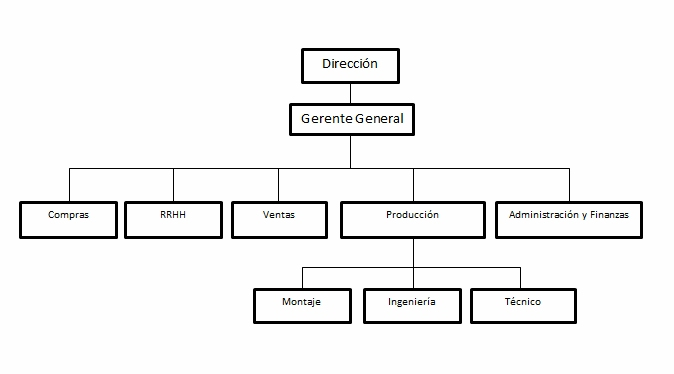
\includegraphics[scale=0.6]{imagenes/inicialHercules.jpg}
					\caption{Organigrama actual Hércules S.A.}
				\end{figure}
						
			\item \textit{Mencionar la descripción de uno de los cargos}\\
			El planeador tiene la responsabilidad de diagramar mes a mes cómo será la producción en función de los avances reflejados por los reportes mensuales (necesidades futuras de los edificios en construcción y departamento técnico).
						
			\item \textit{Mencionar que tipo de configuración estructural se adapta mejor a la organización de referencia}\\
			Uno de los aspectos que podría mejorar la situación sería la estandarización de procesos y productos. Actualmente, la empresa ofrece una amplia variedad de productos, lo cual obliga a fabricarlos casi artesanalmente, por lo que los tiempos de producción son mucho más largos.
			Teniendo en cuenta está consideración y el momento actual que atraviesa la empresa(ya pasados varios años de su creación y volviendose cada vez más grande), la configuración estructural que mejor se adapta a la organización es una burocracia mecánica.
						
			\item \textit{Dibujar el organigrama que refleja el cambio propuesto por ustedes}\\
							\begin{figure}[H]
					\centering
					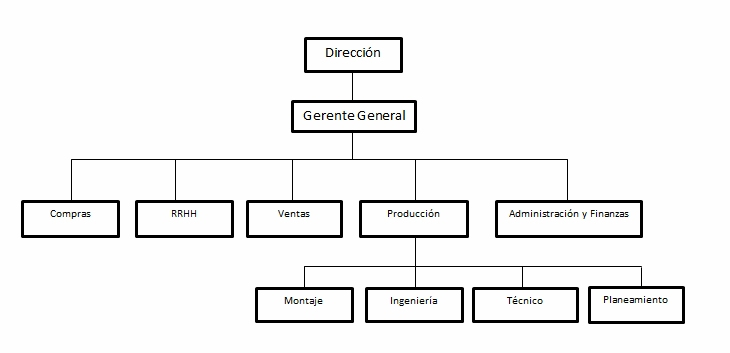
\includegraphics[scale=0.6]{imagenes/FinalHercules.jpg}
					\caption{Organigrama modificado Hércules S.A.}
				\end{figure}
						
			\item \textit{Razonar como la propuesta hecha puede solucionar los problemas planteados}\\

Con la generación de un área de planificación que dependa de Producción, se lograría poner un límite al descontrol en la fechas prometidas por ventas. A su vez esto permitiría una planificación acorde para la producción de manera de empezar a recortar la brecha entre lo prometido por ventas y lo llevado a cabo realmente.\\

Por otro lado, la estandarización de productos y procesos, permitiría mejorar los tiempos y costos de producción. Para no empeorar la imagen entre clientes, podría mantenerse la amplia gama de productos no estandar pero a un precio de venta mucho mayor que los productos estandar y con tiempos de entrega mayores. Esto incentivaría la compra de productos de esta última categoría por parte de los clientes(cliente que se adapta a los productos de la empresa y no empresa que se adapta al cliente). Otra ventaja de esta solución es que se puede predecir mejor que productos se van a vender, por lo que tengo una menor incertidumbre y un stock mucho menos diversificado.

			
			\item \textit{Conclusiones}\\
			Entre las alternativas consideradas que luego fueron descartadas, se encontraron la disminución de las ventas, la tercerización de parte de las producciones y la posibilidad de aliarse con otra empresa del mismo rubro para pasarle parte de la producción(evitando asi el descontento de clientes en caso de no aceptar su pedido). Sin embargo, cada una de las alternativas antes mencionadas presentaban un fuerte impacto en la organización y hubieran significado grandes pérdidas para la compañía.\\
			 Algunas de las causas por las que se las descartó fueron el impacto negativo que podrían tener en la imagen de la empresa en hecho de no responder a ciertos pedidos, el fortalecimiento de un competidor en el caso de la alianza con otra empresa y los grandes costos que podría haber causado la tercerización de parte de la producción.\\
			  Gracias al análisis anterior, concluimos que las soluciones más acertadas resultaron ser la generación de un área de planificación que dependa de producción por un lado y la estandarización de productos y procesos por el otro.
			
			\end{enumerate}
	\subsection{Caso 2: Los Gringos S.A.}
	\subsubsection{Enunciado}
	La empresa Los Gringos SA fue fundada en 1942 por los inmigrantes italianos Aldo y Eduardo Vila. Comenzaron fabricando planchas, suelas y todo tipo de repuestos de goma para la industria del calzado. Este tipo de productos se caracteriza por el empleo de mano de obra intensiva en su fabricación.\newline
	En un principio la fabricación era artesanal y la asumían los propios hermanos Vila en un pequeño galpón rentado junto a 3 obreros. Rápidamente el negocio fue creciendo. Sorteando las distintas crisis nacionales e internacionales gracias al tipo de productos que fabricaban que se adaptaba a los vaivenes de la economía.\newline
	Dicho crecimiento los obligó a una vertiginosa transformación que se tradujo no solo en conseguir y adaptar un predio sensiblemente más grande sino también incorporar tecnología y personal capacitado en las áreas de ventas y técnica.\newline
	Hacia fines de la década del 60 los fundadores son sucedidos en el manejo de la compañía por sus hijos Miriam y Marcelo.
	Miriam Vila es contadora pública nacional y además de ocupar la Gerencia General se hace cargo del área de compras y de la administración en general, mientras Marcelo que no es profesional se ocupó de supervisar todo lo relacionado a las funciones productivas que continuaban a cargo de un técnico formado por los fundadores.
	Simultáneamente Aldo y Eduardo Vila pasaron a formar parte del directorio junto a otros familiares que oportunamente hicieron aportes de capital en el inicio y desarrollo de las actividades empresariales.\newline
	El negocio continuó creciendo año tras año incrementándose el número de clientes todo sustentado por productos de altísima calidad que dieron origen a una prestigiosa marca “Dugom” que en el mercado es sinónimo de garantía.\newline
	Los Gringos SA se caracterizó a lo largo de su existencia por tener una estructura administrativa muy austera y de sus casi 150 empleados tan solo 15 están en las distintas áreas de administración. La estructura administrativa puede representarse mediante el organigrama que se detalla al final de la presentación del caso.\newline
	Aclaración: Existen dos tipos de asesoría jurídica externa, una está relacionada al ámbito estrictamente de la justicia laboral y la otra al de la justicia civil y comercial. Ya comenzado el siglo XXI se produce el tercer recambio generacional ocupando Lucas Vila un licenciado en administración de tan solo 33 años la Gerencia General , su prima Melina Vila de 36 una licenciada en comercialización y publicidad la gerencia de ventas en reemplazo de un ex vendedor con mucha experiencia devenido en gerente en tanto Cesar Zetax un experimentado ingeniero industrial ocupó la gerencia de producción reemplazando al técnico que por casi 45 años había estado a cargo de esas funciones.\newline
	En forma prácticamente coincidente con estos importantísimos cambios y separado por un lapso de dos meses se retiró el ingeniero químico Ricardo Mengos que ocupaba la gerencia técnica, un profesional de 75 años y que por más de 50 brindó sus servicios a la compañía, ingresando en su reemplazo Carolina Vila, hermana de Lucas, una Ingeniera química de 29 años.\newline
	Estos cambios muy profundos en la conducción ahora claramente liderada por gente muy joven y pujante que a pesar de contar con el total apoyo de la familia con fuerte presencia en el directorio cuenta con muy poco recorrido profesional pero a pesar de ello deciden dar otro enfoque a la empresa y entre sus principales decisiones debemos mencionar:\newline
	\begin{enumerate}
	\item Comenzar a fabricar suelas de goma de mayor complejidad para atender el hasta ahora ignorado mercado deportivo (Varios colores combinados en el mismo artículo)
	\item Incursionar en la fabricación de suelas de poliuretano
	\item Incursionar en la fabricación de suelas de PVC
	\item Certificar Normas ISO 9000
	\item Que estos cambios tengan mínimo impacto en la estructuraadministrativa.
	Nota: El proceso detallado en el punto 1 requiere el uso de mano de obra intensiva en tanto los de los puntos 2 y 3 no.		\end{enumerate}
	¿Qué curso de acción aconsejaría seguir al gerente general Lucas Vila a fin de cumplir con todos los puntos enunciados en el término de dos años?
		\newpage
				\begin{figure}
				    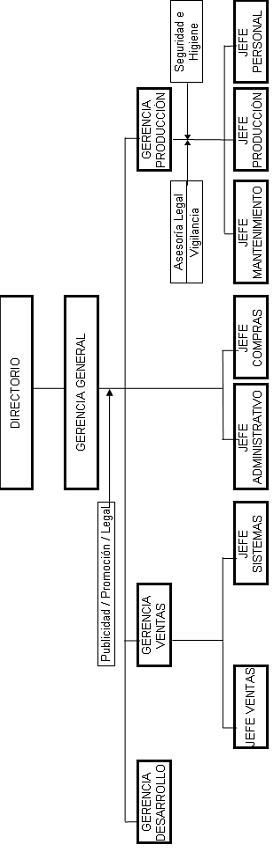
\includegraphics[width=0.3\textwidth]{imagenes/imagenLosGringos.png}
				\end{figure}
				\newpage
	\subsubsection{Preguntas}
	
	\begin{enumerate}
		
			\item \textit{ De acuerdo al enfoque de sistemas, caracterizar a la organización de referencia indicando las entradas, las salidas, la retroalimentación y el ambiente}\\
			
			
			\begin{itemize}
			\item Entradas:
			Materia prima e insumos necesarios para la producciíon.
			\item Proceso:
			Producción de  distintos productos orientados a la industria del calzado.
			\item Salidas:
			Variedad de productos que serán utilizados como insumos del calzado. Por ejemplo las suelas de goma,planchas,etc.
			\item Retroalimentación:
			La retroalimentación se basó en el estudio y la búsqueda de nuevos mercados.
			
			\item Ambiente:
			El ambiente fue variando con los años ya que la competencia en la industria del calzado fue creciendo. Esto obligó a incorporar nuevas tecnologías y personal capacitado técnicamente y así producir productos más complejos que se adaptan a las exigencias del mercado.
			\end{itemize}		
			
			\item \textit{¿Cúal es el problema evidente que enfrenta la empresa}\\
			La empresa sufre constantemente cambios generacionales en la conducción, y  ahora la empresa es liderada por gente muy joven que tiene poco recorrido profesional, jubilando a toda persona con amplio conocimiento y experiencia dentro de la industria.Los nuevos directivos deciden dar otro enfoque a la empresa y necesitan establecer un plan de acción para los objetivos propuestos. Los objetivos son comenzar a fabricar nuevos productos para incorporarse en nuevos mercados,y además certificar las Normas ISO 9000.
			
			\item \textit{¿Cúal es la parte de la estructura que surge como clave?}\\
			La parte identificada como clave es la tecnoestructura, ya que lo que cada directivo nuevo de la empresa lo que busca es la estandarización del trabajo, así como también tener un plan de producción e investigaciones operativas constantes que es lo que le dá el exito a la empresa. \\

			
			\item \textit{¿Cúal es el mecanismo de coordinación preponderante y por qué?}\\
			El mecanismo de coordinación preponderante es la estandarización de los procesos productivos.\\ El crecimiento de la empresa a lo largo del tiempo hizo aumentar la cantidad de empleados lo que requiere a su vez empleados calificados para las tareas técnicas, con el fin de certificar el proceso de producción actual. 
						
			\item \textit{Dibujar el organigrama actual de la companía}\\
			\begin{figure}[!h]
			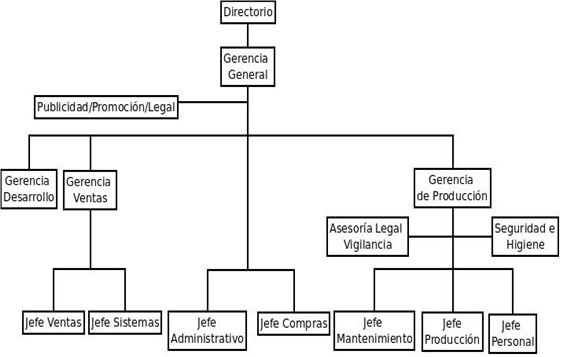
\includegraphics[width=0.75\textwidth]{imagenes/orgaLosGringos.png}
			\end{figure}			
			\item \textit{Mencionar la descripción de uno de los cargos}\\
			A continuación se describirá el siguiente cargo: \textsc{Gerente de Producción}.\\
			El Gerente de Producción debe diseñar, programar y controlar los sistemas de producción. Esto incluye controlar el uso y reposición de tecnología, así como también los métodos de trabajo y la utilización de maquinaria.\\
			Por lo tanto sus tareas serán las siguientes:
			\begin{itemize}
				\item Controlar el Mantenimiento: Esto se refiere no solo a encargarse de que se lleve a cabo las tareas de limpieza del área, sino también cualquier tipo de inconveniente con las maquinarias, nuevas construcciones, etc.
				\item Planeamiento y control de la producción: Para esto deberá contar con personal capacitado, tal cual se ve en el organigrama, como las distintas asesorías.
				\item Fabricación: todo lo que la empresa produzca correrá a cargo suyo y a la vez de sus subordinados.
				\item Control de calidad: La calidad de los productos también son tareas de este área, por lo tanto la gerencia deberá controlarlo. 
			\end{itemize}
			\item \textit{Mencionar que tipo de configuración estructural se adapta mejor a la organización de referencia}\\
			La configuración de la estructura es del tipo burocracia mecánica debido a las características de la empresa:
			\begin{itemize}
			\item Tiene un número considerable de empleados (150 según enunciado).			
			\item Busqueda de certificación de procesos.
			\item Estandarización de procesos de trabajo.
			\item La tecnoestructura es parte central de la estructura de la empresa.
			\item Posee personal calificado y tecnología adecuada al proceso de producción.			
			\end{itemize}

						
			\item \textit{Dibujar el organigrama que refleja el cambio propuesto por ustedes}
		
			
				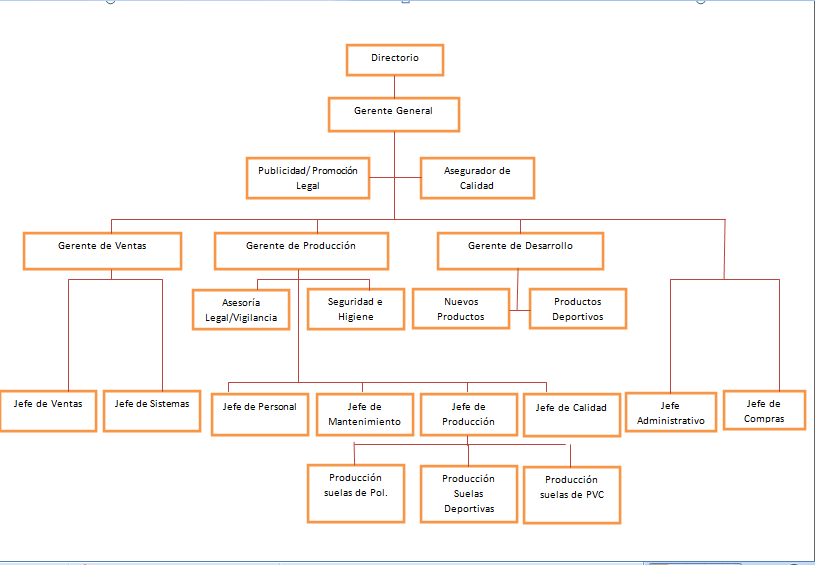
\includegraphics[width=1\textwidth]{imagenes/SolucionPropuestaGringo.png}
				
				
				
						
			\item \textit{Razonar como la propuesta hecha puede solucionar los problemas planteados}\\
			
			En primer lugar se ve claramente que la empresa desea expandir el mercado fabricando nuevos productos.(Suelas de PVC, poliuretano y deportivas). Estos cambios obligan a modificar la estructura de Producción por lo que una idea válidad sería separar las nuevas areas de producción pero dependiendo de la misma jefatura de producción clásica. Además a la gerencia de Desarrollo habría que separarla en 2 partes. La de los productos nuevos y la de los productos deportivos\\
			La otra mejora planteada es la implementación de las normas ISO 9000. Para esto se debe promover un Jefe de Calidad que se encargue del control de los distintos procesos que serán certificados.\\ Además el gerente general debe agregar un nivel de supervisores en la jefatura de producción para lograr una mayor especialización en la  producción de los nuevos productos a desarrollar. Para esto deberán capacitar a los empleados que sean asignados a los nuevos productos.
			

			
			\end{enumerate}
		
	\subsection{Caso 3: La Rapidez}
	\subsubsection{Enunciado}
	La Rapidez S.A. es una empresa distribuidora de productos alimenticios y artículos de limpieza, fundada a principios de la década de los 60; tiene un centro de distribución de unos 10.000 m2, con amplias oficinas en tres niveles, ubicado en un barrio bastante residencial de la ciudad de Buenos Aires, muy cerca de la avenida de circunvalación y del ingreso de dos importantes rutas que unen la ciudad con otros grandes centros de país. El directorio de la empresa está formado por el presidente, Ing. Jorge Fernández, el vicepresidente, Dr. Frederic Johnson, la socióloga Marisa Leal, el contador Mario Aseff y el Lic. David Berenstein. Marisa y David ingresaron al directorio en marzo de 1997 y a los pocos meses plantearon la necesidad de adoptar una política más agresiva con respecto al mercado, sobre todo con medidas concretas respecto de la distribución física. Marisa tiene 29 años, está cursando un posgrado en dirección empresaria y está entusiasmadísima con el  tema de la calidad de servicio; está convencida de que ese tema será de capital importancia para el crecimiento de la compañía y, más aún, que permitirá revelar las diferencias a favor de La Rapidez respecto de las empresas competidoras. Varias charlas con los gerentes de la empresa habían permitido detectar que los mandos medios desconocían totalmente el tema de la calidad de servicio, confundiéndolo con la calidad intrínseca de los productos, la calidad de los envases y embalajes y algunos otros temas bastante difusos.\\Después de un gran esfuerzo por parte de los mencionados, en una reunión de directorio celebrada en octubre de 1999 lograron modificar el punto de vista de Frederic sobre la necesidad de “hacer algo”; decidieron que uno de los caminos posibles era llamar a un grupo consultor y coincidieron en que unos buenos candidatos podrían se Black, Negro \& Noir Consultores Asociados, uno de los cuales había sido compañero de estudios de Frederic y era además viejo amigo de la familia de Jorge. Se convino en llevar a cabo una reunión entre los directores de La Rapidez S.A. y uno de los socios del equipo consultor, donde éste planteó la conveniencia de efectuar un diagnóstico del área de distribución física de la empresa, para luego proponer un plan de acción que debería ser tratado por el directorio antes de iniciar una acción concreta. Aceptada la idea de Noir, le pidieron la propuesta para los primeros días de diciembre a los efectos de poder aprovechar los resultados durante las grandes ventas de fin de año.\\
	A la fecha del estudio La Rapidez contaba con 97 personas en el centro de distribución, más 11 empleados y un inspector; estas 97 personas se subdividían en un jefe, 10 encargados y supervisores, 35 operarios para manipuleo y preparación de pedidos, 10 conductores de autoelevadores y 33 repartidores. La entrega se hacía con 45 camiones, 12 de propiedad de una empresa contratista y 33 fleteros independientes; cada camionero contaba con un acompañante, provisto por la empresa. La Rapidez también tenía sucursales en Mar del Plata, Bahía Blanca, Córdoba y Tucumán. Las provincias patagónicas y las del litoral eran servidas directamente desde Buenos Aires mediante transportes generales en cuyos depósitos se hacían las entregas.
	Los datos que impresionaron a Valery Noir fueron los siguientes: de los 12.325 pedidos de setiembre, 10.089 fueron facturados sin inconvenientes y 2.236 fueron devueltos; una planilla de devoluciones por canal y por causa revelaba que en ese período se habían recibido en devolución el 12\% de los kilogramos despachados en la ciudad de Buenos Aires y alrededores; se consignaban una serie de causas (11), que se transcriben:\\
	\begin{itemize}
	\item	Portón cerrado
	\item Dirección incompleta
	\item Calle intransitable
	\item Mercadería en mal estado
	\item Fuera de horario
	\item No está pagador
	\item No se cargó
	\item Anulado por cliente
	\item Pedido repetido
	\item No lo pidió
	\item Mal facturado
	\end{itemize}
	En 4 días, sobre 2504 despachos, 380 correspondieron a entregas menores de u\$s 50.-, totalizando el 0,46\% de la facturación, 882 facturas eran menores de u\$s 100.-con el 1,7\% de la facturación, 1245 entregas eran menores de u\$s 150.-, con el 3,2\% del total; y 1571 eran menores de u\$s250.-y representaban el 5,4\% del total. Los pedidos se preparan para su entrega el día siguiente, pero el último día hábil del mes se lleva a cabo un inventario físico, que demanda 20 personas, por lo cual las entregas del primer día hábil del mes siguiente se reducen en volumen. El total de ventas está en el orden de los 7 millones de dólares USA por mes, con un volumen de 6.000 toneladas. El stock al 30 de setiembre era de 4.574 ton. Medidos en días de venta, los inventarios mostraban este detalle:\\
	\begin{tabular}{||l | c ||}
	\hline
	\hline
	Fideos y harina & 18\\
	\hline
	Yerba & 10 \\
	\hline
	Mermeladas & 349\\
	\hline
	Mermeladas importadas & 100 \\
	\hline
	Wiskey & 54\\
	\hline
	\hline
	\end{tabular}\\
	Los porcentajes de clientes activos respecto de los totales, separados por tipo de empresa y por zona, daban un cuadro desparejo, con un máximo de 69,4\% para mayoristas de Buenos Aires, 12,2\% para Córdoba y 35,8\% para supermercados de Buenos Aires. El gerente de comercialización, Jorge Arbusto, no dejaba de repetir que la imagen de la empresa entre sus clientes era mala; el gerente de distribución, Rubén Rozansky, decía a quién quisiera escucharlo que él no se sentía responsable de la situación, mientras el de planificación comercial, Carlos Brown, opinaba que a la empresa le faltaba una política comercial y que él poco podía hacer frente al desorden general que presentaba la compañía.\\
	Valery se reunió también con el gerente administrativo, el Lic. Fritz Crysler, para reunir datos acerca de los costos de distribución, los originados por las devoluciones, los de personal, alquileres y gastos fijos. Fritz le cuenta que los costos de distribución están subdivididos en numerosos ítems que se generaban en distintas áreas de la empresa y que controlaban distintos sectores de diferentes gerencias. Mario había estado buscando desde hacía varios meses una fórmula que permitiese integrar los distintos componentes del costo de distribución, y dijo que no estaba seguro de que los gastos de cobranza y los costos financieros del stock debían ser tomados en cuenta al momento de calcular los costos de distribución. Con Fritz inquirió también cómo funcionaba el sistema de verificación de créditos, la respuesta fue que lo hacía un grupo formado por Guillermo García y Amalia Sánchez, que trabajaba en el segundo piso, con una computadora que no estaba conectada con la red interna, todos los pedidos pasaban por esa oficina y las conformidades demoraban entre 24 y 48 horas; luego eran transferidos al área de control de inventarios, luego de lo cual pasaban a su preparación. También se discutió el tema de la veracidad de las causas de devoluciones, registradas en los informes; verificando la documentación apareció por ejemplo un caso de un producto que el cliente consideró como de precio excesivo, pero el camionero registró como “no recibido por falta de dinero”; otro cliente había efectuado dos pedidos iguales, para recibirlos en distintas fechas, se los entregaron el mismo día, pero el camionero indicó “devuelto sin causa”; ningún repartidor había indicado nunca las fallas por llegadas tarde al cliente.\\
	Los tiempos de detención de los vehículos en los clientes fueron también motivo de observación, considérese que no había comenzado aún la utilización generalizada de los equipos GPS, que registran todas las variables y que en la oportunidad en que se escribe este texto, año 2011, ya cubrirían todos estos problemas sin mayor intervención humana. El promedio de tiempos de detención, en todos los vehículos a lo largo de 4 días, fue de 27 minutos, el mínimo de 11 minutos y el máximo de 39 minutos.
	
	\subsubsection{Diagnóstico}
	Los problemas detectados en la empresa fueron:
	\begin{itemize}
	\item Se desconoce el concepto de calidad de servicio por parte de los mandos medios, provocando un servicio de baja calidad.
	\item La gran cantidad de devoluciones de productos genera grandes perdidas, las cuales en general no son identificadas.
	\item Las causas de las devoluciones no estan bien informadas por lo que muchas veces se tiene información erroneo de ellas, haciendo muy dificil su reducción.
	\item No se tiene certeza de la forma en la que se deben calcular los costos de Distribución, haciendo imposible su análisis y estudio, en busca de su reducción. 
	\item La verificación de créditos funciona de una forma muy precaria, con sólo 2 personas encargadas de esta tarea y con una única computadora desconectada de la red interna de la empresa, lo que generá muchas demoras y errores que con una red interna podrían solucionarse.
	\item Hay una mala comunicación entre los distintos sectores de la empresa y, en algunos casos, no se escuchan los diagnósticos y propuestas que realizan las gerencias.
	\item Se cree que hay un gran desperdicio de tiempo en las detenciones de los vehículos en los clientes ya que existen diferencias muy notorias entre los tiempos de detención.
	\item Falta de una correcta supervisión en varias areas de la empresa y análisis de los reportes generados 
	\end{itemize}
	Todos estos incovenientes están llevando a que la imagen de la empresa entre sus clientes se cada vez peor.	
	
	\subsubsection{Posibles Soluciones}

Algunos aspectos que podrían mejorar la situación actual de la empresa son:

\begin{itemize}
\item Capacitaciones del personal para lograr que los mandos medios reconozcan la importancia de un servicio de calidad y puedan entender en qué aspectos trabajar para llevarlo a cabo.
\item Preparación de pedidos con más de un día de anticipación, para disminuir las demoras en las entregas ocasionadas por no tener listo los pedidos a la hora de distribuirlos. De esta manera también podría amortizarse la reducción de entregas que se ocasiona el primer día de cada mes, debido a las 20 personas requeridas para el inventario físico del último día de cada mes. 
\item Creación de un departamento de costos y/o contratación de personal especialzado en dicha area encargado de la tarea de recompilar los costos implicados en los distintos sectores de la organización, en busca de una visión global en materia de costos y de una reducción de los mismos.
\item Fortalecimiento de la coordinación y comunicación entre los distintos miembros de la línea media para permitir la resolución conjunta de problemas y el crecimiento de las distintas areas en un mismo sentido, con objetivos comunes.
\item Recopilación de las causas de las devoluciones por parte del acompañante del camionero, el cual es empleado de la empresa y debería esta mejor capacitado en esta tarea que el camionero.
\item Supervisión directa de los camioneros y acompañantes para estar seguro que los informes generados por estos sean verídicos y precisos, de modo que se pueda crear un plan de acción para reducir las devoluciones. Además, con una supervisión más estricta podría ayudar a reducir las demoras en los lugares de detención cuando estas no sean por causas de fuerza mayor, ya que los camioneros se sentirian más controlados.
\item Mejoramiento del mecanismo utilizada para la verificación de créditos a través de la implementación de un sistema conectado a la red interna de la companía que agilice esta tarea y a través del controlamiento de area por parte de la gerencia de administración.

\end{itemize}


\begin{comment}
\begin{thebibliography}{99}

\bibitem{INT06} Intel Technology \& Research, ``Hyper-Threading Technology,'' 2006, http://www.intel.com/technology/hyperthread/.

\bibitem{HEN00} J. L. Hennessy and D. A. Patterson, ``Computer Architecture. A Quantitative
Approach,'' 3ra Edición, Morgan Kaufmann Publishers, 2000.

\bibitem{LAR92} J. Larus and T. Ball, ``Rewriting Executable Files to Mesure Program Behavior,'' Tech. Report 1083, Univ. of Wisconsin, 1992.

\end{thebibliography}
\end{comment}
\end{document}
